\documentclass[10pt,a4paper]{article}

\usepackage[utf8]{inputenc}
\usepackage[margin=1.2in]{geometry}
\usepackage[french]{babel}
\usepackage{amsmath}
\usepackage{amsfonts}
\usepackage{graphicx}
\usepackage{hyperref}
\usepackage[nottoc, notlof, notlot]{tocbibind}
\hypersetup{colorlinks=true,citecolor=black,filecolor=black,linkcolor=black,urlcolor=black}
\setlength{\parindent}{0.6cm}
\setlength{\parskip}{0.10cm}
\usepackage[automark]{scrpage2}
\usepackage{color, colortbl}
\usepackage[table]{xcolor}


\pagestyle{scrheadings}

\ihead[]{Équipe Navigation}
\ohead[]{Plan de Développement Qualité}



\begin{document}
\pagestyle {plain}

\begin{titlepage}


\newcommand{\HRule}{\rule{\linewidth}{0.5mm}} 

\center

\textsc{\Large Université Paul Sabatier}\\[1cm] 

\includegraphics[scale=0.3]{UPS.jpg}\\[0.6cm] 


\textsc{Master Intelligence Artificielle et \\ 
Reconnaissance des Formes \\ Master Robotique : Décision et Commande}\\[3cm] 

\HRule \\[0.4cm]
{ \huge \bfseries Plan de Développement Qualité}\\[0.4cm] 
\LARGE Navigation Autonome de Robot Mobile

\HRule \\[1.5cm]
 

\begin{minipage}{0.4\textwidth}
\begin{flushleft} \large
\emph{Auteur:}\\
\href{mailto:brefel.hugo@gmail.com}{Hugo \textsc{Brefel} }  \\
\href{mailto:sylvain31g@free.fr}{Sylvain \textsc{Guillaume} } \\
\href{mailto:luc.rubio.lr@gmail.com}{Luc \textsc{Rubio} } \\
\href{mailto:salaheddineghamri@gmail.com}{Salah Eddine \textsc{Ghamri} } \\
\href{mailto:beauhaire.pierre@gmail.com}{Pierre \textsc{Beauhaire} }  
\end{flushleft}
\end{minipage}
~
\begin{minipage}{0.4\textwidth}
\begin{flushright} \large
\emph{Tuteur:} \\
\href{mailto:lerasle@laas.fr}{Frédéric \textsc{Lerasle}}\\
\href{mailto:michael.lauer@laas.fr}{Michaël \textsc{Lauer}} \\
\href{mailto:taix@laas.f}{Michel \textsc{Taix}}
\end{flushright}
\end{minipage}\\[5cm]


\includegraphics[scale=0.3]{laas.png} \\[1.1cm] 

\large 7 novembre 2016
% laaaaaaaaaaaaaaaaaaaaaaaaaaaaaaaaaaaaaaaaaaaaaaaaaas
 

\end{titlepage}

\newpage


\subsection*{Suivi du document}

\begin{center}
    \begin{tabular}{| l | l | l | l | l |}
    \hline
     \rowcolor{gray} Nom du document & Version Majeure & Date de création & Dernière version \\ \hline
    PDDQ & 2.0 & 10/01/2018 & 18/01/2018 \\ \hline
    \end{tabular}
\end{center}


\subsection*{Auteurs du document}

\begin{center}
    \begin{tabular}{| l | l | l | l |}
    \hline
    \rowcolor{gray} Rédaction & Intégration & Relecture & Validation Interne \\ \hline
    Équipe & Hugo Brefel & Hugo Brefel & Hugo Brefel \\ 
     & Sylvain Guillaume & Sylvain Guillaume & Sylvain Guillaume \\
     & Luc Rubio & Luc Rubio & Luc Rubio \\
     & Salah Eddine Ghamri & Salah Eddine Ghamri & Salah Eddine Ghamri \\
     & Pierre Beauhaire & Pierre Beauhaire & Pierre Beauhaire \\ \hline
    \end{tabular}
\end{center}

\subsection*{Validation du document}

\begin{center}
    \begin{tabular}{| l | l | l | l |}
    \hline
     \rowcolor{gray} Validation & Nom & Date & Visa \\ \hline
    & & & \\
     \hline
    \end{tabular}
\end{center}

\subsection*{Liste de diffusion}

Le plan de développement qualité est diffusé à l'ensemble des clients et des intervenants externes au projet.

\subsection*{Historiques de révision}

\begin{center}
    \begin{tabular}{| l | l | l | l |}
    \hline
     \rowcolor{gray} Version & Modification apportée & Auteur & Date \\ \hline
    2.0 & Création et intégration du document & Pierre Beauhaire & 18/01/2018\\
     & & Luc Rubio & \\
     \hline
     
    \end{tabular}
\end{center}

\newpage
\tableofcontents
\newpage
	

\section{Introduction}
\label{sec:introduction}

La structure et le contenu de ce Plan de Développement Qualité de Projet ont été élaborés dans le cadre du projet « Navigation autonome de robots mobiles » proposé aux étudiants de deuxième année du Master « Intelligence Artificielle et Reconnaissance des Formes » et « Robotique : Décision et Commande » de l'Université Paul Sabatier à Toulouse.

Il a pour objectif la définition et la description des différentes dispositions à mettre en œuvre pour un développement optimal du projet afin d’en assurer la qualité et d’atteindre les résultats attendus. Plus précisément, sont déterminés, d’un commun accord :
\begin{itemize}
\item l’organisation globale du projet 
\item le plan de gestion et de développement du projet
\item les droits et les devoirs de chaque partie prenante
\item la répartition des responsabilités entre les organismes dans la structure
\item les plans de développement et de gestion du projet
\item les outils qui seront adoptés 
\end{itemize}

Après acceptation par le client, ce plan deviendra le document contractuel applicable en matière de gestion et d’assurance qualité entre le Titulaire et le Client durant la durée totale du projet. Le responsable qualité s’assurera qu’il est effectivement appliqué. Il ne pourra subir aucune modification sans accord préalable du Client. En cas de divergence entre les exigences et le plan qualité, les exigences s’appliqueront en priorité.

% -------------------------------

\section{Présentation du projet}
\label{sec:presentation}

\subsection{Contexte}

\subsubsection{Master IARF et RODECO}

Le master « Intelligence Artificielle et Reconnaissance des Formes » (IARF) a comme objectif de former des professionnels de haut niveau capables de concevoir des solutions à des problèmes complexes utilisant des méthodes avancées de représentation et de traitement de l’information, faisant appel à des techniques d’intelligence artificielle (IA), de reconnaissance des formes (RF) et d’apprentissage automatique, appliqués notamment au traitement d’images et à la robotique. 

Le master « Robotique : décision et commande » (RODECO) a pour vocation de promouvoir des connaissances dans le domaine de l’automatique par des enseignements avancés autour de la robotique, de l’informatique et de la commande des systèmes. Ces compétences permettent d’aborder des problématiques très actuelles comme la robotique industrielle haute performance où les aspects commande sont fondamentaux et la robotique  de service où la décision et la perception tiennent une place essentielle. Suivant ce raisonnement, deux blocs de spécialisation sont proposés en M2 : 

\begin{description}
\item [Robotique et décision] qui propose un renforcement des aspects « informatique » (intelligence artificielle, reconnaissance des formes, dialogue homme/machine), vision par ordinateur et robotique  mobile. Cette spécialisation donne les compétences nécessaires pour appréhender le domaine de la robotique de service ;
\item [Robotique et commande] qui se focalise sur le développement et l’implantation de commandes avancées pour la robotique. Cette spécialisation donne donc les compétences nécessaires pour élaborer des solutions évoluées de contrôle/commande pour la réalisation de tâches robotique haute performance.
\end{description}

Au cours de cette deuxième année, les étudiants acquièrent une double compétence en Automatique et Informatique et les capacités requises pour modéliser, analyser, concevoir et réaliser des systèmes automatiques complexes, autonomes et/ou embarqués où sont impliqués la perception (capteurs), l’analyse (traitement de signal, audio, image, vidéo), le raisonnement et la décision (incertitude, reconnaissance de formes, contraintes) et de l’action (commande, robotique).
  
\subsubsection{Contexte du projet}

Le projet de Master 2 permet de mettre en commun et en pratique les connaissances acquises dans ces trois parcours dans un but commun. En l’occurrence, sur le projet « Navigation autonome de robots mobiles », Hugo, Sylvain et Pierre font partie du parcours IARF, Luc est issu de la spécialité Décision de RODECO et enfin, Salah Eddine, de la spécialité Commande.

Le projet est décomposé tout le long de l'année en tranches W, de 3 et 4 semaines, en alternance avec des blocs de cours B.

\newcolumntype{g}{>{\columncolor{gray}}c}
\begin{table}[ht]
\centering
\begin{tabular}{g|c|g|c|g|c}
\hline
 Cours1 & Release1 & Cours2 & Release2 & Cours3 & Release3 \\ 
\hline
 6 sem. & 3 sem. & 5 sem. & 3 sem. & 6 sem. & 3 sem. \\ 
 & 23/10 - 10/11 &  & 18/12 - 22/12 &  & 12/03 - 31/03 \\
 & & & 10/01 - 19/01 & & \\
\hline
\end{tabular}
\end{table}

\subsubsection{Objectif}

Actuellement le robot peut se déplacer dans une salle et estimer à peu près sa position sur une carte préétablie en utilisant des amers (AR-code).
Les objectifs du projet vont, dans un premier temps, être de pouvoir asservir le robot sur l’AR-code, d’améliorer l’estimation de la localisation du robot via le filtre de Kalman et qu’il puisse réaliser des déplacements dans un environnement comprenant plusieurs salles.
Nous allons également nous intéresser à la façon dont la carte représentant l’environnement du robot est créée (jusqu’ici elle était préétablie) et allons essayer de rendre la création et la mise à jour de la carte dynamique. Ceci notamment pour que le robot soit capable de détecter des obstacles qui ne sont pas sur la carte initiale de l’environnement.


\subsubsection{Entrées}
\begin{itemize}
\renewcommand{\labelitemi}{\mbox{\ooalign{$\checkmark$\cr\hidewidth$\square$\hidewidth\cr}}}
\item Cahier des charges
\item Documentations
\end{itemize}

\subsubsection{Sorties}
L'objectif du projet est de répondre à un cahier des charges divisé en 4 étapes incrémentales. Le projet étant amené à être réutilisé par la suite par d'autres étudiants, la qualité du produit est primordiale.

\begin{itemize}
\renewcommand{\labelitemi}{$\square$}
\item Code propre, fonctionnel et surtout facilement réutilisable 
\item Documentation
\item Robot opérationnel qui effectue les tâches demandées
\item Manuel Utilisateur
\end{itemize} 

\subsubsection{Limites}
\begin{itemize}
\item Incrémentation des solutions : difficulté d'anticiper les solutions et problèmes des étapes suivantes
\item Cours de vision 2D et de navigations en B2 et vision 3D en B3
\end{itemize} 

\subsection{Parties-prenantes}

\subsubsection{MOE} 
\begin{minipage}[t]{0.30 \textwidth} 
Hugo \textsc{Brefel} \\
\href{mailto:brefel.hugo@gmail.com}{brefel.hugo@gmail.com} \\
Spécialité IARF \\[0.3cm]
Sylvain \textsc{Guillaume} \\
\href{mailto:sylvain31g@free.fr}{sylvain31g@free.fr} \\
Spécialité IARF \\[0.3cm]
Salah Eddine \textsc{Ghamri} \\
\href{mailto:beauhaire.pierre@gmail.com}{salaheddineghamri@gmail.com} \\
Spécialité Commande
\end{minipage} 
\hfill
\begin{minipage}[t]{0.46\textwidth} 
Pierre \textsc{Beauhaire} \\
\href{mailto:beauhaire.pierre@gmail.com}{beauhaire.pierre@gmail.com} \\
Spécialité IARF \\[0.3cm]
Luc \textsc{Rubio} \\
\href{mailto:luc.rubio.lr@gmail.com}{luc.rubio.lr@gmail.com}   \\
Spécialité Décision
\end{minipage} 

\subsubsection{MOA}
\begin{minipage}[t]{0.46 \textwidth} 
Frédéric \textsc{Lerasle} \\
\href{mailto:lerasle@laas.fr}{lerasle@laas.fr} \\
Équipe RAP, LAAS - CNRS \\[0.3cm]
Michel \textsc{Lauer} \\
\href{mailto:michael.lauer@laas.fr}{michael.lauer@laas.fr} \\
Équipe TSF, LAAS - CNRS
\end{minipage} 
\hfill
\begin{minipage}[t]{0.46\textwidth} 
Michel \textsc{Taix} \\
\href{mailto:taix@laas.fr}{taix@laas.fr} \\
Équipe GEPETO, LAAS - CNRS
\end{minipage} 

\subsubsection{Intervenants externes}
\begin{minipage}[t]{0.46\textwidth} 
Cyril \textsc{Briand} \\
\href{mailto:briand@laas.fr}{briand@laas.fr} \\
Coach
\end{minipage} 

\subsection{Contraintes}
\noindent La réalisation du projet est régie par certaines contraintes citées ci-dessous : 
\begin{itemize}
\item Robot TurtleBot
\item Planning du Master et ses jalons 
\item Connaissances partielles selon les périodes de projet
\end{itemize} 

\subsubsection{Exigences}
Les clients ont spécifié plusieurs exigences :
\begin{itemize}
\item Se déplacer dans un environnement connu à l'avance par le robot, composé de différentes salles.
\item Utiliser les amers dans le but de se localiser.
\item Éviter les obstacles dynamiques.
\end{itemize} 

% -------------------------------


\newpage
\section{Organisation du projet}
\label{sec:organisation}

\subsection{Cycle de développement}

Le développement du projet se fera selon Scrum, une méthode Agile dédiée à la gestion de projet. Cette méthode, basée sur les stratégies itératives et incrémentales, permettra de produire, à la fin de chaque « sprint », un résultat achevé et validé, pour avoir une version fonctionnelle à tout moment. Cette démarche correspond bien au cahier des charges où les étapes sont à la fois itératives et incrémentales.

Pour chaque sprint, la période initiale permettra de faire le point sur les éléments techniques du départ du projet et d'établir une liste des points à préciser ou à compléter, à savoir les charges de travail et le calendrier associé.

Scrum se différencie des autres méthodes de développement par ses avantages qui font de ce procédé une réponse à certains problèmes fréquemment rencontrés dans le développement logiciel. Pour éviter l’effet tunnel, la communication restera permanente entre les membres de l’équipe mais aussi entre l’équipe et le client, permettant une meilleure coopération à l’intérieur de l’équipe Scrum. 

\begin{figure}[!h]
  \centering
  \noindent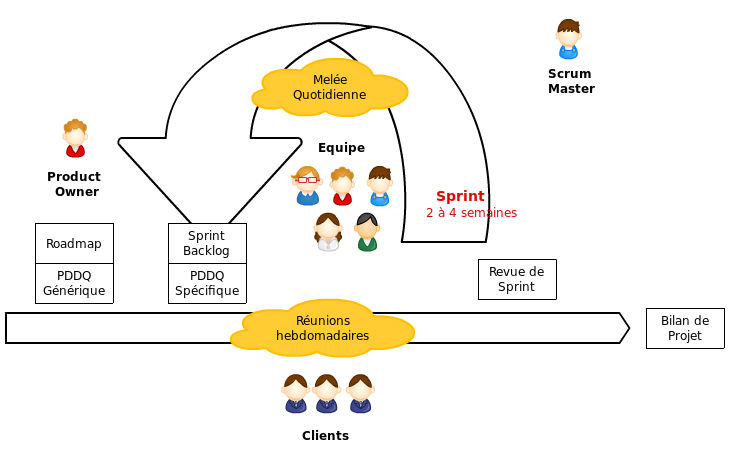
\includegraphics[width=\textwidth]{scrum.png} 
  \caption{Schéma Méthode Scrum}
\end{figure}

\subsection{Sprints}

\noindent Le projet est divisé en 3 étapes définies par le client : 

\begin{description}

\item [Étape 1] Se familiariser avec l'environnement de travail ROS et prendre en main les travaux déjà effectués par l'équipe précédente.

\item [Étape 2] Réaliser une tâche de navigation dans un environnement supposé connu et sans obstacles pour atteindre un amer final en se déplaçant d’amer en amer (QR code : amer 2D) afin de ne pas se perdre et en optimisant un critère (distance, temps, commande,....).

\item [Étape 3] Réaliser une tâche de navigation dans un environnement supposé connu et avec obstacles statiques et dynamiques pour atteindre une position finale en se déplaçant d’amer en amer (QR code : amer 2D) afin de ne pas se perdre et en optimisant un critère (distance, temps, commande,....).

\end{description}

La première étape a pour objectif de prendre en main les différentes ressources à notre disposition. Nous avons également étudié les différentes erreurs qui pouvaient apparaître lors de l'utilisation d'un Turtlebot : erreurs sur l'odométrie lors du mouvement du robot en ligne droite ou en rotation, erreurs sur la détection des amers; tout cela dans le but d'obtenir une quantification des erreurs.

La deuxième étape a pour but la réalisation de la navigation d'un TurtleBot d'un point A à un point B dans un environnement connu, sans obstacles. La rencontre d'amers permet au robot de compenser ses erreurs de trajectoire et ainsi de se relocaliser sur la carte.

A la fin et entre chaque étape, une étude des limites et des problématiques de la prochaine étape est demandée.


\newpage
\section{Arbre produit}

Un arbre produit, ou \textit{Product Breakdown Structure} donne une liste exhaustive des différents livrables du projet, de manière hiérarchisée. Il permet d’avoir une vue claire des différentes fonctionnalités à développer, de décrire l’architecture logicielle et matérielle du produit à livrer, et d’en prévoir les coûts. Dans le cadre de notre projet de navigation, l’aspect budgétaire ne sera pas abordé puisqu’il s’agit d’un projet dans le cadre de la formation.
La figure suivante présente l’arbre produit du projet de navigation. Les parties encadrées correspondent aux nœuds de l'arbre, c’est à dire les groupes de fonctions à développer, tandis que les parties non encadrées correspondent aux feuilles, autrement dit aux fonctions elles-mêmes.
L’arbre produit de notre projet de navigation est décomposé en cinq parties :

\begin{description}
\item  [Perception] : Décrit l’ensemble des fonctionnalités permettant l’identification à partir d’une image. Plusieurs fonctions interviennent. Le robot va chercher à détecter des amers. Un traitement est également appliqué sur la carte de l'environnement : une érosion pour enlever le bruit sur l'image, une dilatation pour compenser l'érosion...
La détection des obstacles devra tenir compte des différentes méthodes utilisées au cours de ce projet : le nuage de points, l’étude laser, les différentes méthodes de segmentation, etc...
\item [Localisation] : Décrit les fonctions nécessaires à la navigation autonome du robot. Le robot estime sa position grâce à la reconnaissance des amers et à la triangulation du filtre de Kalman.
\item [Décision] : Décrit les fonctions nécessaires aux différentes décisions que le robot doit prendre pour naviguer jusqu'au point but. Le robot calcule un graphe de connexité reliant les points du nuage de points. Il détermine ensuite le chemin avec le coût le plus intéressant jusqu'à la position finale. Afin d'avoir une trajectoire continue, des courbes de Bézier sont calculées pour lisser la trajectoire.
\item [Action] : Concerne toutes les fonctions correspondant au domaine de la commande robotisée permettant le respect des consignes (atteindre un amer...), la réalisation des mouvements, et les contraintes cinématiques.
\end{description}

\begin{figure}[!h]
  \centering
  \noindent\centerline{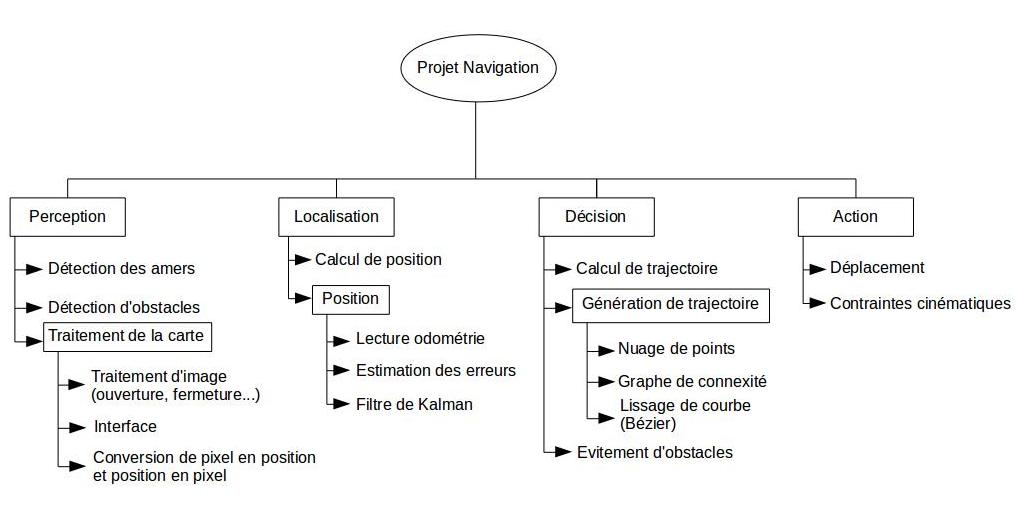
\includegraphics[scale=0.3]{Arbre_produit.png}}
  \caption{Arbre Produit}
\end{figure}

\newpage
\section{RoadMap}

\begin{figure}[!h]
  \noindent\centerline{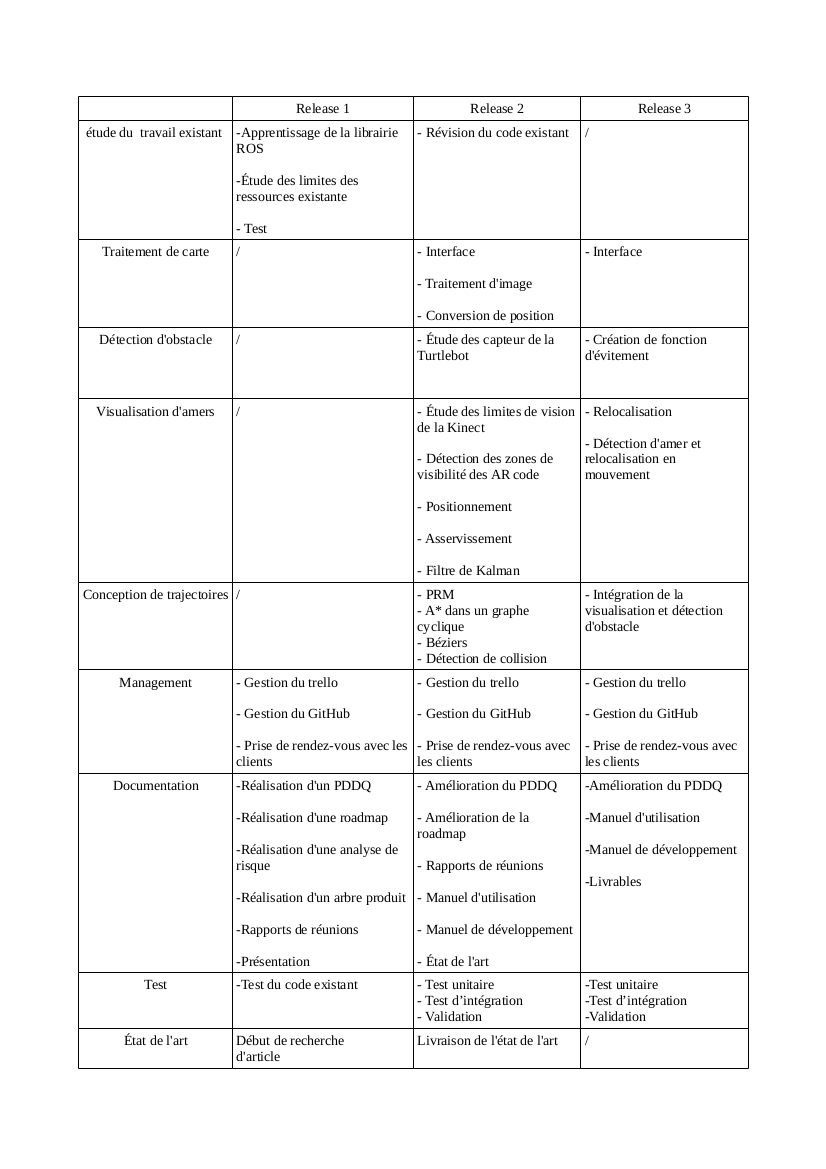
\includegraphics[scale=0.5]{Roadmap.png}}
  \caption{Roadmap}
\end{figure}

\newpage
\section{Planning}
\label{sec:planning}

\subsection{Backlog}

Un \textit{backlog} est une liste de fonctionnalités ou de tâches jugées nécessaires et suffisantes pour la réalisation satisfaisante du projet.
Il permet à la fois d'avoir une représentation visuelle du travail restant à réaliser, mais aussi d'évaluer rapidement l'avancement de chacune des tâches.

\begin{figure}[!h]
  \centering
\noindent\centerline{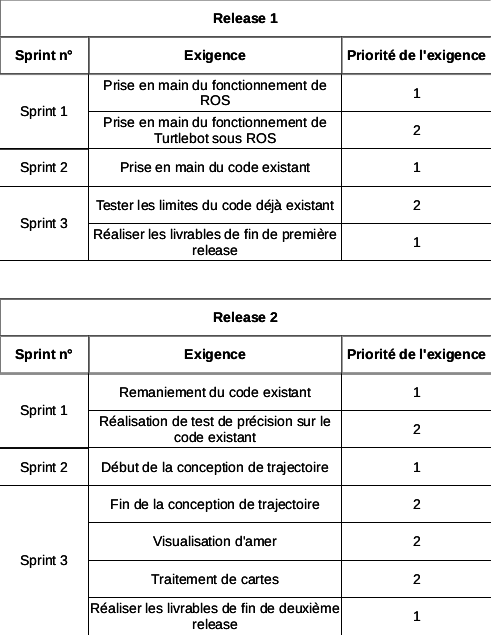
\includegraphics[scale=0.3]{Backlog.png}}
  \caption{Backlog des Release1 et Release2}
\end{figure}

\subsection{Planning général}

\begin{figure}[!h]
  \centering
\noindent\centerline{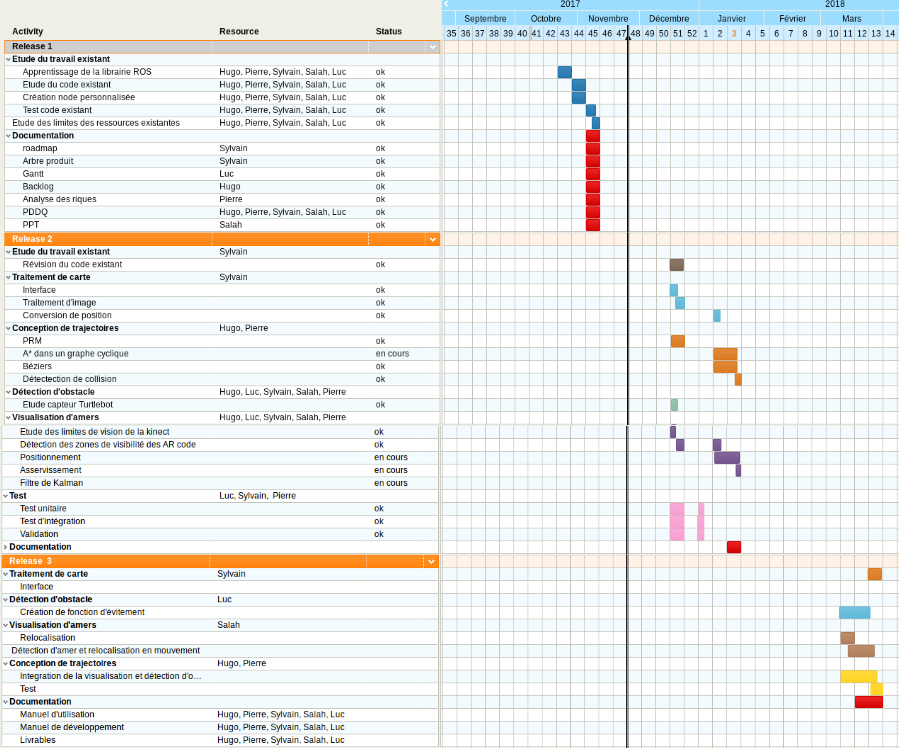
\includegraphics[scale=0.3]{Gantt.png}}
  \caption{Gantt du projet}
\end{figure}


\subsection{Livrables}

\subsubsection{Pour le client}

\begin{description}

\item [Release1] du 23/10 au 10/11 : 
\begin{itemize}
\item Backlog de Release1
\item Plan de Développement et de Qualité V1 : 16/11/2017
\end{itemize}

\item [Release2] du 18/12 au 19/01  : 
\begin{itemize}
\item Backlog de Release2
\item État de l'Art : à la fin du Release2
\item Plan de Développement et de Qualité V2 : 19/01/2018
\end{itemize}

\item [Release3] du 12/03 au 31/03  : 
\begin{itemize}
\item Backlog de Release3
\item Code et Manuel Utilisateur : fin de Release3
\item Bilan de projet : à la fin de Release3
\item Présentation et démonstration publique : fin de Release3
\end{itemize}

\item [Tout au long du projet] : 
\begin{itemize}
\item Compte-rendus de réunions 
\end{itemize}
\end{description}

\subsubsection{Pour les intervenants externes}
\begin{itemize}
\item Compte-rendus de réunions 
\item Plan de Développement Qualité
\end{itemize}


\subsection{Conclusion du projet}

Ce plan qualité vise à assurer que les dispositions prises par l’équipe pour obtenir la qualité du logiciel définie en accord avec les clients soient respectées. Avec le même objectif, le responsable qualité, soutenu par toute l’équipe, sera en charge de vérifier que les engagements pris dans le présent document auront été appliqués tout au long de l'avancement de ce projet.

Les membres de l'équipe projet sont tenus de se conformer aux dispositions décrites dans le plan de développement qualité. Le non-respect des prescriptions du plan de développement qualité constaté donne lieu à un plan d'action curatif pour corriger les effets du dysfonctionnement et éventuellement à un plan d'action préventif pour éviter que celui-ci ne se reproduise. Ce dernier plan peut entraîner une modification du plan qualité. L’utilisation de ce plan doit permettre un total succès du projet :

\begin{description}
\item [Succès du produit] : avoir un produit final qui satisfait les besoins des utilisateurs, qui a le niveau de qualité requis (tests, code propre et commenté) et qui puisse être évolutif (générique) et réutilisable (documentations).
\item [Succès de la démarche] : satisfaire les demandes du client dans les délais. Respecter les méthodes établies et le planning.
\end{description}

Le projet et les résultats obtenus seront décrits dans le bilan et exprimés lors de la présentation orale et de la démonstration publique. 

% ----------------------------

\newpage
\section{Assurance qualité}

\subsection{Organisation interne}


L'organisation de notre projet suit une configuration Agile.
Nous avons réparti les rôles dans l'équipe afin de respecter cette organisation :
\begin{itemize}
\item Scrum Master (Pierre Beauhaire) : Il est responsable du processus de développement.
\item Product Owner (Hugo Brefel) : Il représente le client au sein de notre équipe. Il dirige l'ordre de développement des fonctionnalités en maximisant la satisfaction du client.
\item Responsable Technique (Sylvain Guillaume) : Il veille au respect des spécifications et des contraintes de mise en œuvre.
\item Responsable Qualité (Luc Rubio) : Il effectue les tests unitaires et les tests de validation. Il est responsable de la qualité du projet, et doit donc veiller au respect des exigences.
\item Équipe de développement : Ensemble des membres du projet.
\end{itemize}
En ce qui concerne la communication interne au groupe, des mêlées sont organisées par le Scrum Master tous les jours vers 10h. Ces réunion sont courtes et ne doivent pas dépasser les 15 minutes. Chaque membre du groupe fait le point sur ce qu'il a effectué la veille, ce sur quoi il travaillera le jour de la réunion et sur les éventuels obstacles liés à ses activités.


\subsection{Organisation externe}

La communication avec les clients se fera généralement par courrier électronique. Les clients pourront alors répondre à l’équipe via l’adresse mail du groupe mise à leur disposition. Des réunions seront également prévues afin de tenir informés les intervenants sur l’avancement du projet. Des réunions supplémentaires pourront également être organisées si cela s’avère nécessaire. Chaque réunion sera prévue au moins 2 jours à l’avance et donnera lieu à un compte rendu de réunion. Ces comptes rendus seront envoyés par courriel, dont l’objet sera identifié, et ils seront rédigés à partir des formulaires fournis en Annexe. Ces documents seront soumis à l’approbation dans les trois jours. De plus, toutes les informations relatives au projet, quelle que soit leur nature seront accessibles immédiatement dans nos espaces de travail (voir 7.3).

\subsection{Outils}

\subsubsection{Développement}
\begin{description}
\item [Système d'exploitation : Ubuntu 14.04 LTS et ROS]
\item [Git] : Logiciel libre de gestion de versions. Nous l'utilisons pour la gestion de nos sources mais aussi pour gérer la rédaction collaborative de nos documents.
\item [Github] : Hébergeur de notre dépôt Git. L'interface Web fournit également un accès à des outils de gestion du code. Une liste d'Issues sera utilisé pour discuter des modifications effectuées dans les codes. Un wiki est également accessible via cette interface.\\ \href{https://github.com/Projet-M2-TurtleBot-UPS}{[lien vers le dépôt GitHub]} 
\end{description}

\subsubsection{Documentation}
\begin{description}
\item [LaTeX - TexMaker] : LaTeX est un langage de rédaction de document. Il permet la rédaction de document et l'intégration de plusieurs parties facilement. Nous avons décidé de choisir une distribution LaTeX commune pour s'assurer que les documents produits soient homogènes (encodage, caractères spéciaux etc)
\end{description}

\subsubsection{Espace de travail}
\begin{description}
\item [Tom's Planner] : Logiciel de gestion de projet. Il nous permet de modéliser dans le temps l'ensemble des tâches liée au projet ainsi que leur relation entre elles.
\item [Trello] : Outil de gestion de projet en mode « Tableau de tâches ». Il nous permet d'organiser la distribution et la réalisation des tâches. Il sert également comme vecteur d'information sur la gestion du projet en général (liens des outils, documents importants… etc.).\\ \href{https://trello.com/projetturtlebot}{[lien vers le tableau Trello]}
\item [Google Mail] : Service de messagerie électronique. Il est utilisé pour l’ensemble de nos échanges internes ou externes au projet.
\end{description}
 
\subsection{Standards}

\subsubsection{Gestion des documents}

Chaque document produit par le groupe projet devra comporter une page de garde reprenant les éléments nécessaires à leur suivi :
\begin{itemize}
\item Informations générales de suivi :
\begin{itemize} 
	\renewcommand{\labelitemii}{$\cdot$}
	\item Nom du document
	\item Version
	\item Date de création
	\item Date de modification
\end{itemize}
\item Auteurs du document
\item Auteur et date de la validation du document pour la version en cours.
\item Historique de révision
\end{itemize}

\noindent Processus de production des documents :
\begin{itemize}
\item Rédaction des parties du document par l'ensemble des auteurs concernés ;
\item Ajout des rédactions par \textit{commit} sur le dépôt Git. 
\item Fusion et résolution des conflits. Ajout des corrections si nécessaire ;
\item Validation finale d'une version du document. \textit{Tag} de version sur le dépôt Git ;
\item Envoi ou diffusion du document aux destinataires concernés ;
\item Archivage du document.
\end{itemize}

Il peut être nécessaire de répéter plusieurs fois la partie rédaction, ajout et fusion afin d'obtenir une version du document convenable.

\subsubsection{Objet des e-mails}

Pour des raisons de suivi, l'ensemble des e-mails est envoyé à plusieurs destinataires chacun travaillant dans des domaines différents. Pour faciliter la recherche et l'identification du contenu des e-mails, nous avons décidé de respecter la forme d'objet suivante : 

\verb|[Projet NAV - Thème] Objet du mail|

\subsubsection{Entête des fichiers}
L'entête de chaque fichier source doit être complétée afin d'expliquer leur comportement. Elle doit être mise à jour au fur et à mesure des évolutions du fichier qu'elle décrit.
Chaque entête doit permettre de comprendre facilement et rapidement les fonctionnalités codées.
Voici une liste non exhaustive des éléments à renseigner :
\begin{itemize}
\item Méthode/Fonction
\begin{itemize} 
	\renewcommand{\labelitemii}{$\cdot$}
	\item \verb|D:| Descriptif
	\item \verb|A:| Auteur(s)
	\item \verb|E:| Description des paramètres
	\item \verb|S:| Donnée(s) renvoyée(s)
	\item \verb|R:| Donnée renvoyée
	\item \verb|F:| Exceptions et/ou code(s) d'erreur(s) renvoyé(es)
\end{itemize}
\item Classe
\begin{itemize} 
	\renewcommand{\labelitemii}{$\cdot$} 
	\item Descriptif
	\item Auteur(s)
\end{itemize}
\end{itemize}

Il est recommandé de commenter au maximum le code afin de faciliter la phase de développement du projet.

\subsubsection{Nommage}

Les fichiers suivent le nommage de leur classe respective.
Pour les fichiers C++ c'est le suffixe .cpp qui sera utilisé. Pour les headers C++ le suffixe .hpp sera utilisé.
\begin{description}
\item [Classes] :
\begin{itemize}
\item Première lettre en majuscule 
\item Mélange de minuscule, majuscule. 
\item Première lettre de chaque mot en majuscule
\item Donner des noms simples et descriptifs 
\item Éviter les acronymes 
\item N’utiliser que \verb|[a-z][A-Z]| et \verb|[0-9]|
\end{itemize}

\item [Variables] : 
\begin{itemize}
\item Première lettre en minuscule
\item Mélange de minuscule, majuscule avec la première lettre de chaque mot en majuscule 
\item Donner des noms simples et descriptifs 
\item N’utiliser que \verb|[a-z][A-Z]| et \verb|[0-9]|
\end{itemize}


\item [Constantes] :
\begin{itemize}
\item Tout en majuscule 
\item Séparer les mots par des underscore
\item Donner des noms simples et descriptifs 
\item N’utiliser que \verb|[A-Z]| et \verb|[0-9] |
\end{itemize}

\end{description}

\subsubsection{Découpage du code}

Il est important que le code soit suffisamment découpé. La taille des fichiers ne devrait pas excéder 1000 lignes et chaque fonction (ou méthode) ne devrait pas dépasser la centaine de lignes au grand maximum. Les headers et les fichiers source séparent les déclaration des définitions.

L'indentation doit être strictement respectée et doit correspondre à un espacement de 4 caractères. La taille des lignes ne doit pas dépasser 80 caractères.


\subsubsection{Workflow}

Voici une description du \textit{workflow} utilisé pour réaliser les tâches de développement de notre projet :
\begin{itemize}
\item La branche \textit{master} contient uniquement un système complet en état de fonctionner. Elle est protégée en écriture par le Scrum Master.
\item La branche \textit{develop} est notre branche de travail par défaut.
\item Pour travailler sur une nouveauté, on travaille directement sur la branche \textit{develop} ou on créé une nouvelle branche à partir de la branche \textit{develop} lorsque la fonctionnalité développée demande au moins un jour de travail.
\item Lorsque la branche de travail est prête, on ouvre une \textit{Pull Request} pour demander une intégration à la branche master au Scrum Master.
\item Validation et/ou corrections des modifications. Une fois que cela est fait on fusionne dans la branche \textit{master}.
\item Déploiement du code de la branche \textit{master} sur le système.
\end{itemize}

Il est également important d'alimenter le \textit{wiki} lorsqu'un membre du groupe estime qu'une information importante concernant les développements doit être partagée aux utilisateurs et/ou aux membres du projet. La forme de rédaction est libre mais chaque page doit être référencée avec un titre précis et explicite sur le contenu qu'elle présente.

Il est conseillé de respecter le format suivant pour les préfixes des \textit{commit} sur le dépôt Git :
\begin{itemize}

\item \verb|ADD| : Ajout de fichiers, de méthodes, d'une configuration, d'un texte \ldots etc...
\item \verb|ENH| : Amélioration d'un élément déjà présent
\item \verb|RM| : Suppression d'un fichier, d'une méthode, d'une classe, d'un texte \ldots etc...
\item \verb|BUG| : Correction d'un bug.
\item \verb|TEST| : Relatif aux tests.
\item \verb|DOC| : Relatif à la documentation.
\end{itemize}

Il est nécessaire que l'ensemble des membres du projet utilisent la liste d'\textit{Issues} pour pouvoir effectuer et archiver les différents discussions sur le code du projet. Il est possible d'ouvrir et de fermer ces \textit{issues}. Lorsqu'un \textit{commit} est en rapport avec une \textit{issue} il doit être relié avec celui-ci (i.e. \verb|BUG : add method close #12| ce commit ferme automatiquement l'\textit{issue} numéro 12).

\newpage
\section{Analyse des risques}
L’analyse des risques projet se doit d’être menée dès le tout début de la phase de lancement, afin d’identifier au plus tôt et de la manière la plus exhaustive possible les éléments qui pourraient avoir une influence négative sur le déroulement du projet. Cette analyse est destinée à évoluer tout au long de notre projet.
Les risques seront synthétisés et classés dans un tableau avec pour chacun sa définition, sa probabilité,
sa gravité, ses causes et effets, ainsi que les actions préventives et correctives à mettre en oeuvre pour y pallier. On définira ainsi la criticité de chaque risque.

\begin{figure}[!h]
  \centering
  \noindent\centerline{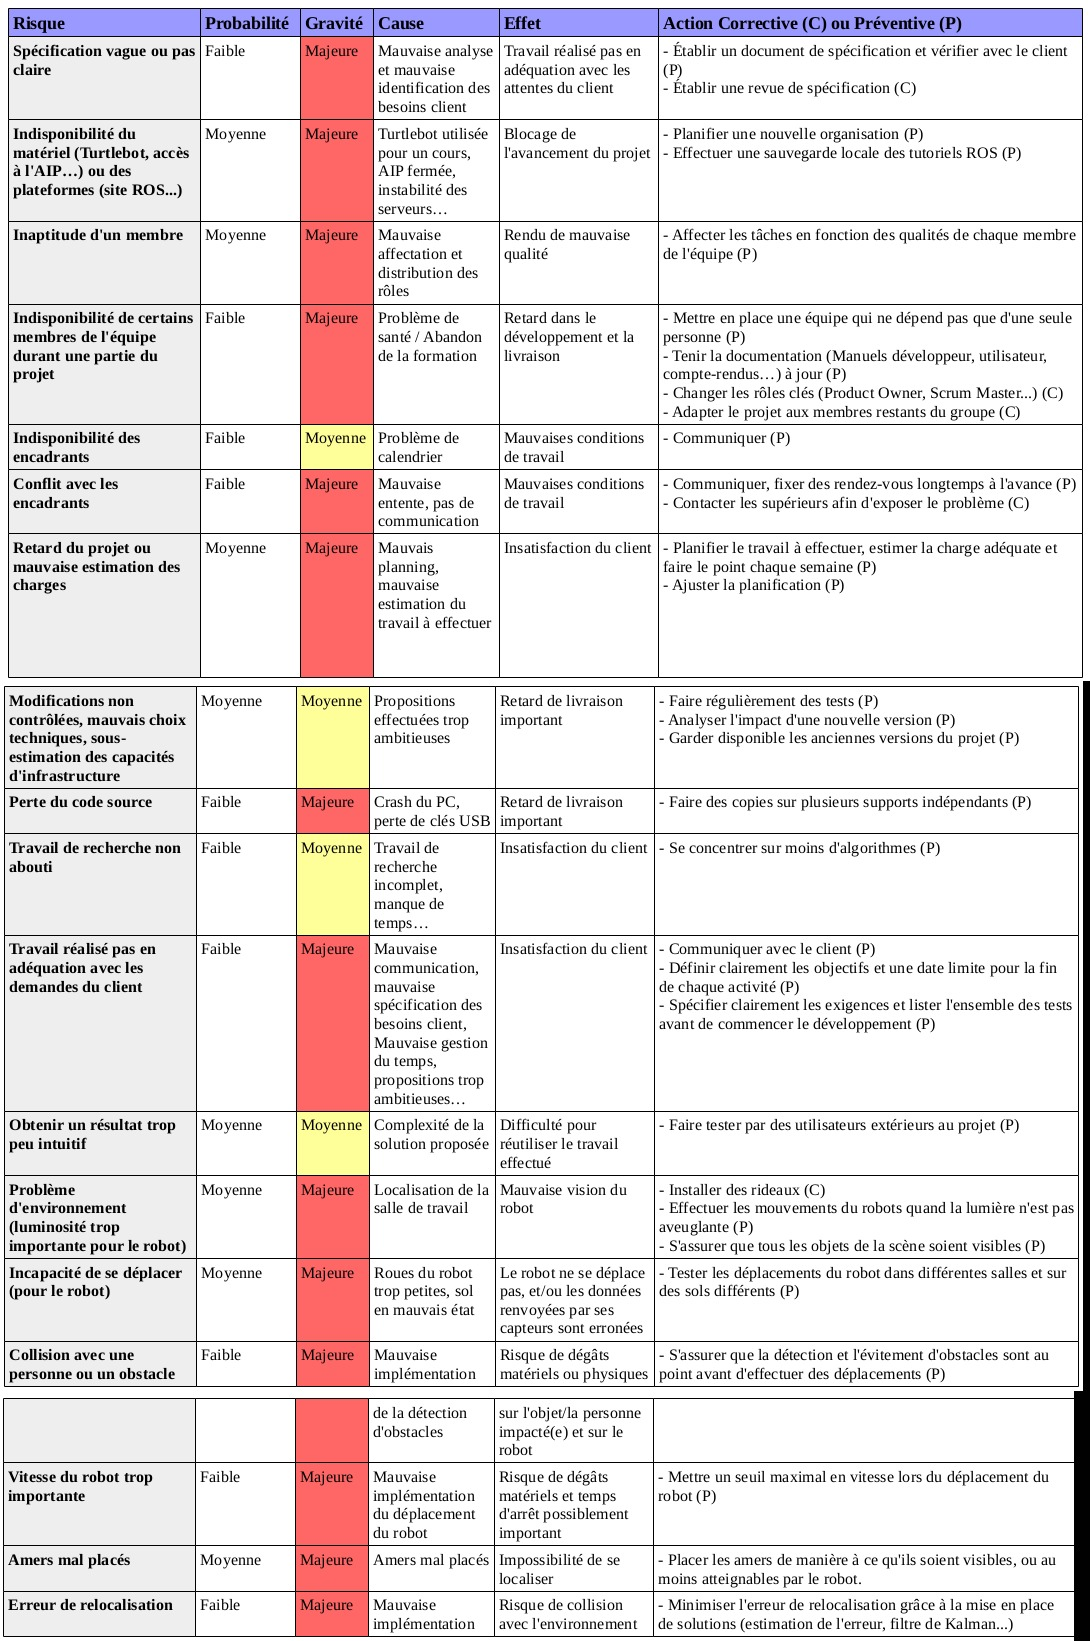
\includegraphics[scale=0.32]{Analyse_des_risques.jpg}}
  \caption{Analyse des risques}
\end{figure}

\newpage
\section*{ANNEXE}

\noindent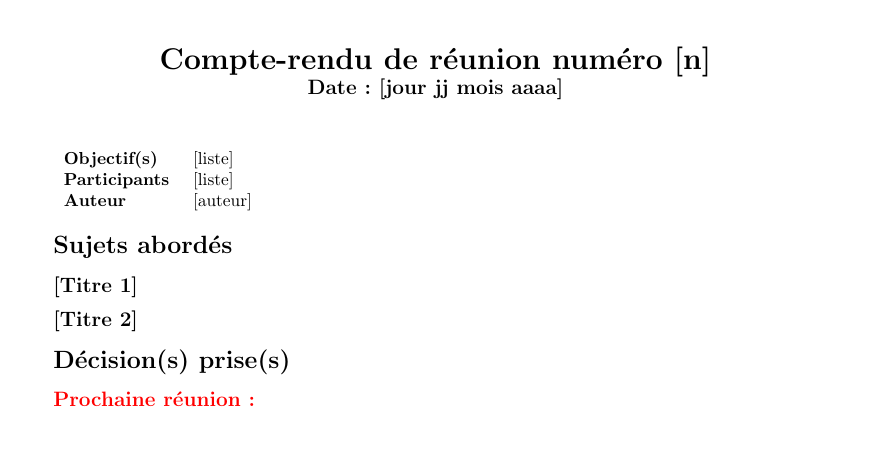
\includegraphics[width=\textwidth]{tmp-cr.png} 



\end{document}

